\chapter{Methodology}
The research concept of the thesis is divided as follows. First, a systematic literature review (\acrshort{slr}) will be conducted according to \cite{vomBrockeJan2019TDgs, Webster2002AnalyzingTP}. Second, knowledge from the first part will be applied to the project RAPADO. The implementation part of this master thesis follows an agile development approach. RAPADO use cases for zero-knowledge proof protocols are investigated, conceptualized, and evaluated, considering aspects found in previously examined literature and preliminary work at the Department of Information Systems at Freie Universit{\"a}t Berlin. The application of acquired technical and theoretical knowledge is at focus, while the use cases implemented can be exchanged in the future during further project research. 

\section{Systematic Literature Review}
The initial and current status and results of project RAPADO are discussed. From this analysis, potential use cases and design requirements for the application of zero-knowledge proofs are derived. Following the requirement to accumulate knowledge within the project to build expertise in blockchain-based development for the aviation industry, the literature survey focuses on designing zero-knowledge proofs and theoretical foundations. Opportunities and challenges are displayed considering practical examples. The second part of the research concept is implementing a zero-knowledge application for  data attestation and verification, focusing on the demonstration of technical mechanisms.

Previous research at the Department of Information Systems concludes with conceptual solutions and a decentralized application for aviation industry  documentation, centering storage, and traceability \citep{ZedelJ}. As a result, use cases of uploading, storing, and trading aircraft spare parts certificates were given. This research extends previous findings. However, it takes a new perspective by further investigating possible use cases for \acrshort{zkp}s to automate verification processes, preserve data confidentiality, and suggest suitable data formats. The results are expected to represent the broader research project, i.e., beyond previously used software.

The \acrshort{slr} focuses on zero-knowledge proofs with the scope of classification, opportunities, challenges, evaluation methods, and examples in practice. The design of zero-knowledge proofs needs to be examined from a theoretical perspective. Application domains and use cases applicable to the research project are at focus, which excludes topics of cryptocurrencies and embedded systems. This survey aims to provide an extensive overview of the design and implementation of zero-knowledge proofs and to bring out practical and critical implications. The final search string is derived from a concept map (Figure \ref{fig:con_map}), and the selected literature is shown in a concept matrix, with headers displayed in Figure \ref{fig:concept_matrix} and the entire matrix in Appendix \ref{Appendix A}.

\begin{figure}[hbt]
	\centering
	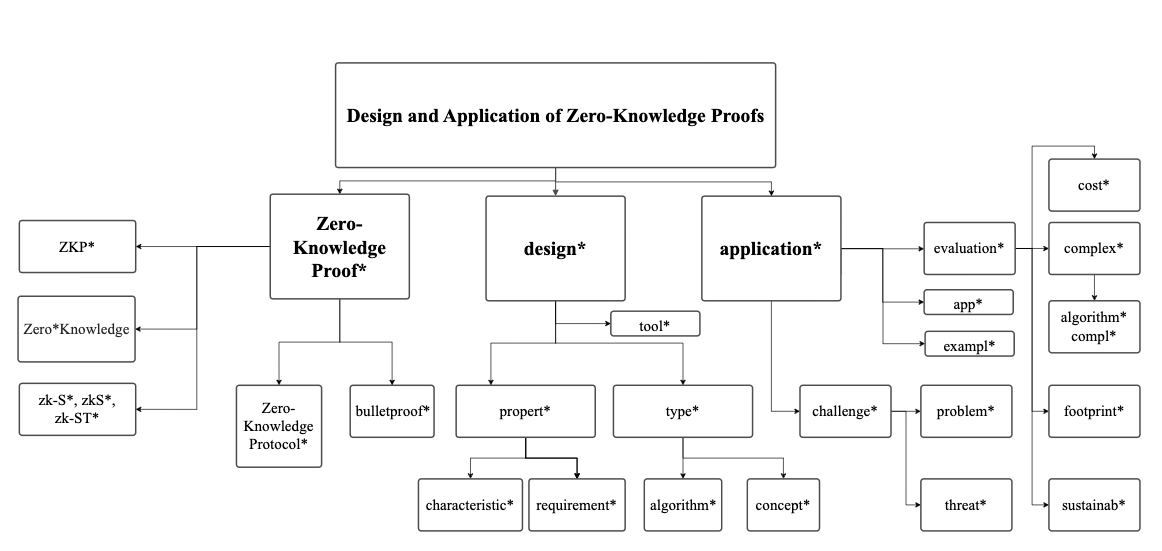
\includegraphics[width=0.99\textwidth]{Pictures/con_map.png}
	\caption{Concept Map - Compression of Main Topics and Relations as Basis for Final Search String}
	\label{fig:con_map}
\end{figure}

The research question concerns topics of computer science, mathematics, and information systems. For the search, the databases Web of Science (WoS), Association of Computing Machinery (ACM), zbMATH, arXiV, Association of Information Systems (AIS), and Institute of Electrical and Electronics Engineers (IEEE) were queried. Articles were searched in Title, Keywords, and Abstract, with date restrictions back to 2018 (WoS) and 2006 (ACM). The following search string was used: (("ZKP*" OR "Zero-Knowledge*" OR "zero*knowledge*algorithm*" OR "zero*knowledge*protocol*" OR "zero*knowledge*proof*" OR "zkS*" OR "zk*SNA*" OR "zk*STA*" OR "zk*STO" OR "bulletproof*") AND ("application*" OR "example*" OR "app*") AND ("carbon*footprint*" OR "*complexity*" OR "evaluation*" OR "cost*" OR "sustainab*" OR "environment*") AND ("challenge*" OR "threat*" OR "problem*")). After deduplication, the search resulted in 580 hits further condensed according to the following approach. First, the result was filtered by English or German resources with more than or equal to five citations three times or higher past 180 days of usage (560 hits). The next exclusion criteria were applied in Title and Keywords (396 hits), Abstract (319 hits), and Full-text (80 hits), of which backward/forward search added another 20 hits. 

\begin{figure}[hbt]
	\centering
	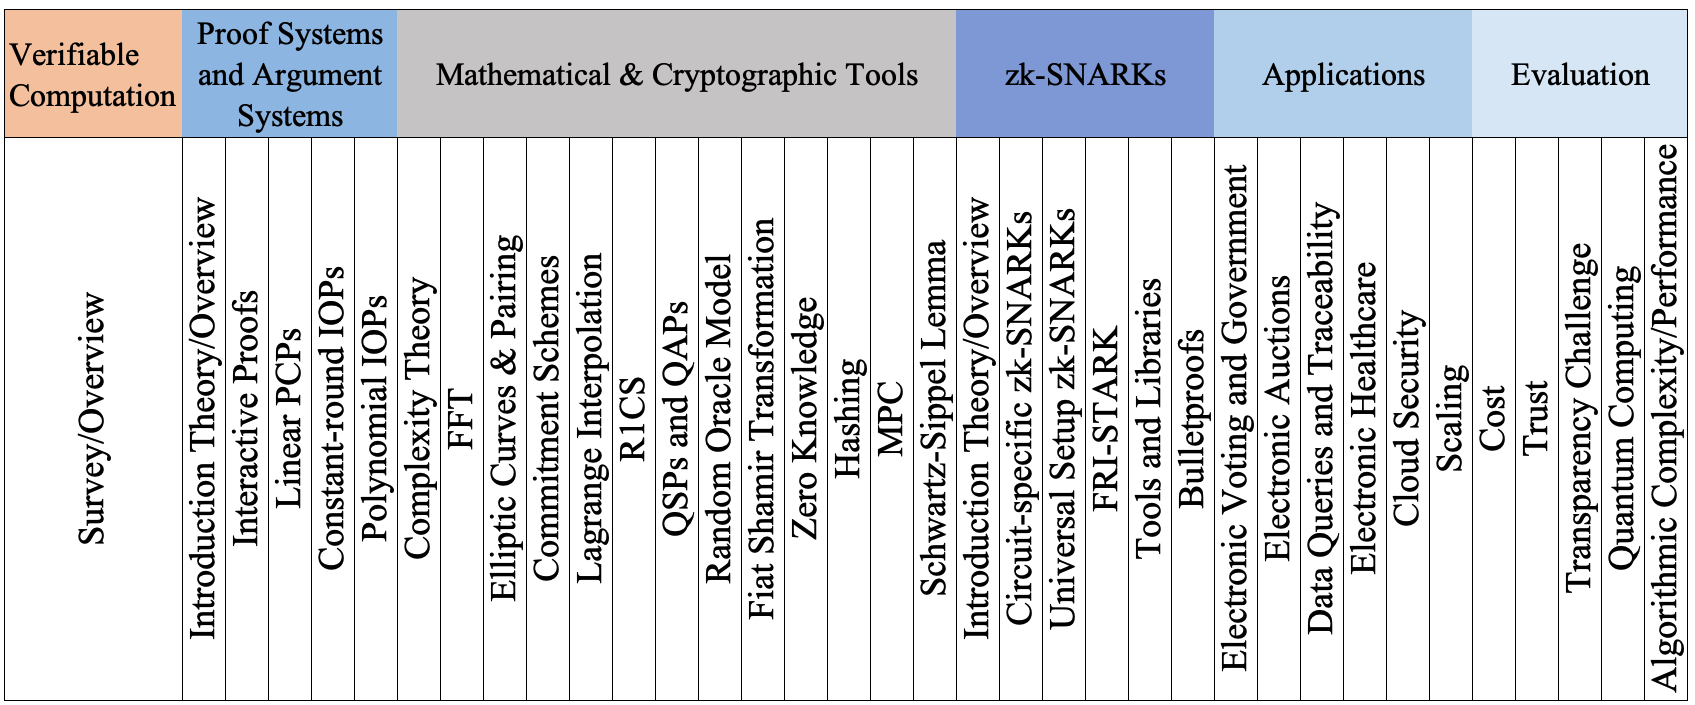
\includegraphics[width=1.0\textwidth]{Pictures/concept_matrix_headers.png}
	\caption{Concept Matrix - Outcome Summary of the Systematic Literature Review}
	\label{fig:concept_matrix}
\end{figure}

The results of the survey are categorized as follows. 
\begin{itemize}
    \item Algorithm design topics: Zero-knowledge proofs are designed by combining proof systems and cryptographic means to achieve specific characteristics. Proof systems are examined and defined, linking and presenting cryptographic tools within the scope of building zero-knowledge argument systems in the area of applicable blockchain-based solutions.
    \item Widely used and performative zero-knowledge proofs are described in more detail, i.e., algorithms of specific \acrshort{zksnark}s, \acrshort{zkstark}s, and Bulletproofs.
    \item Selective literature is reviewed according to the identified problem domains: Electronic Voting and Government, Electronic Auctions, Data Queries and Traceability, Electronic Healthcare, Cloud Security, and Rollups.
    \item Opportunities and challenges are discussed and aligned by evaluating and comparing the different algorithms qualitatively through literature review and quantitatively through complexity analysis.
\end{itemize}

\section{Implementation and Evaluation}
The results of this master thesis are three artifacts, each satisfying a requirement in project RAPADO. The requirements are derived from previous work at the Department of Information Systems at Freie Universit{\"a}t Berlin and workshops held within the project consortium. The development of artifacts is conducted agilely, focusing on the demonstration of the technical application of zero-knowledge proofs via prototyping \citep{mci/Wilde2007}. Table \ref{tab:summary_artifacts} summarizes the three artifacts and their implementation approach.
\setlength{\tabcolsep}{2ex}
\renewcommand{\arraystretch}{1.5}%
\begin{table}[htb]
	\centering
	    \caption{Summary of Artifacts and Implementation Approaches}
		\begin{tabular}{|m{0.001\linewidth} | m{0.11\linewidth} | m{0.35\linewidth} | m{0.35\linewidth} |}
		\hline
		\textbf{}& \textbf{Artifact} & \textbf{Short Description} & \textbf{Implementation} \\ \hline
            1&Groth16 Example \newline Calculation & Step-wise computation of Groth16 protocol by taking a simple polynomial as an example. The goal is to create a reference document to underline zk-SNARKs functionality, corresponding to the requirement of accumulating expertise on the topic within the project. & Developed during the research phase on zk-SNARKs theory and functionality by taking a simple proof example and following the Groth16 protocol steps \citep{Groth2016OnTS}. \\  \hline
            2&\acrshort{zkdapp}  \newline Attestation & Zero-knowledge decentralized application to attest to  data of parts and create a trusted, verified process. & Agile development focuses on demonstrating the \acrshort{plonk} \acrshort{zksnark}s functionality and practical implementation with circom and snarkjs. First, feedback is collected and implemented. \\ \hline 
            3&Zero-Knowledge Data \newline Structure & Motivated by recurring comments during workshops and project consortium meetings, this is the first architecture prototype to enable further discussion of effective data formats and digitization of spare parts and corresponding documents. & Analyzing similar efforts in other alternative fields of research \citep{sedlemeirgrenenergy}, key insights are combined with results from the literature survey to implement first ideas and approaches to utilize zero-knowledge proofs to create effective data formats and standards for the future of aviation. \\ \hline 
	\end{tabular}
\label{tab:summary_artifacts}
\end{table}

The algorithms studied in Chapter 4 are evaluated according to their complexity. Artifact 1 represents a reference document to understand zk-SNARK functionalities. Artifact 2 is evaluated through the first feedback collection from the project partner. Enhancements are implemented and summarized in Chapter 5. Artifact 3 is evaluated by revisiting project and design requirements to reassess current and future project needs.